\chapter{Generating Geodesics}
\label{chp:generating-geodesics}

This chapter will describe two main algorithms for generating the geodesics of the Fabrykowski-Gupta group.
Further, these algorithms will collect the geodesics into their respective equivalence classes, that is, they will collect together geodesics which represent the same group element.

This chapter will begin with a section that shows two propositions about geodesic equivalence classes in the Fabrykowski-Gupta group.
These propositions will then be used in later sections to improve the complexity of the geodesic generating algorithms therein.

In \cref{sec:brute-force}, the brute force method will be described.
This method makes use of the word problem (see \cref{alg:word-problem}) to check if a given word is a geodesic by comparing it with words of lesser length.

In \cref{sec:sortingMethod}, a more efficient method will be described, with the full details of this method being provided in \cref{apx:modified-mergesort}.
This method is based on a modified sort algorithm, which is made possible by the ability to compare words (see \cref{alg:compare-words}) in the Fabrykowski-Gupta group in the sense of a total order.

In \cref{sec:theoretic-methods}, two additional methods will be briefly mentioned.
These methods will not be explored in detail as they are not the focus of this thesis, but rather a potential avenue for future research and improvement.
Both of the methods are based on the existence of a hash function from the words in $X^\ast$ to $\mathbb{N}$ which possesses some particular properties.

This chapter will then conclude, with \cref{sec:complexity-comparison}, by providing the full complexities of the brute force and sorting-based methods; and giving a comparison of these two algorithmic complexities.

%\newpage
\section{Preliminaries}

This section will introduce two propositions related to geodesic equivalence classes of the Fabrykowski-Gupta group.
These propositions will allow for improvements to the time complexity of the algorithms which will be outlined in the following sections.

\begin{proposition}
	\label{prop:geodesic-subwords}
	Let $w = w_1 w_2 \cdots w_n$ be a geodesic word, where each $w_j \in X$.
	Then, the sub-word $v = w_2 w_3 \cdots w_n$ is also a geodesic, and each word in the geodesic equivalence class of $v$ will begin with a letter in $\left\lbrace w_2^{\pm 1} \right\rbrace$.
\end{proposition}

\begin{proof}
	Let such a length $n$ geodesic $w$ be given.
	
	Let $v = w_2 w_3 \cdots w_n$, then clearly $v$ is a length $n-1$ geodesic as otherwise there would exist some shorter word $v^\prime =_\mathbb{G} v$, which would then imply that $w_1 v^\prime =_\mathbb{G} w$ is of length less than $n$, contradicting the assumption of $w$ being a length $n$ geodesic.
	
	Since $w$ is a geodesic, it is known from \cref{prop:geodesics-in-alt-form} that $w$ is in the alternating form.
	
	Suppose, for contradiction, that there exists a geodesic $u = u_2 u_3 \cdots u_n \in \equivClass{v}$ such that $u_2 \notin \left\lbrace w_2^{\pm 1} \right\rbrace$, and thus $u_2 \in \left\lbrace w_1^{\pm 1} \right\rbrace$ as $w$ is in the alternating form.
	
	Then, $w_1 u_2 u_3 \cdots u_n$ is the same (with respect to its action) as $u_2^\prime u_3 \cdots u_n$ for some $u_2^\prime \in \left\lbrace 1,w_1^{\pm 1}\right\rbrace$.
	Hence, $w_1 u =_\mathbb{G} w$ is of length at most $n-1$, which contradicts $w$ being a geodesic of length $n$.
\end{proof}

\begin{corollary}
	\label{cor:extending-geodesics-criterion}
	Given a geodesic equivalence class $\equivClass{v}$ containing a word $v = v_1 v_2 \cdots v_n$ where each $v_j \in X$.
	If $av$ is a geodesic for some $a \in X$, then each word in $\equivClass{v}$ begins with either $v_1$ or $v_1^{-1}$.
\end{corollary}

\begin{proposition}
	\label{prop:extending-geodesics}
	\ \\
	Let $v = v_1 v_2 \cdots v_n$ be a length $n$ geodesic for which each word in $\equivClass{v}$ begins with a letter in $\left\lbrace v_1^{\pm 1} \right\rbrace$.
	
	Then, with $w = a v$ for some letter $a \in X$ where $a \notin \left\lbrace v_1^{\pm 1} \right\rbrace$, either
	\begin{itemize}
		\item $w$ is a length $n+1$ geodesic; or
		\item $w$ is equivalent (with respect to its action) to a length $n$ geodesic.
	\end{itemize}
\end{proposition}

\begin{proof}
	Let such a $v \in X^\ast$ and $a \in X$ be given.
	
	Let $u \in X^\ast$ be a geodesic word such that $u =_\mathbb{G} w$ where $w = av$.
	Notice then that $a^{-1} u =_\mathbb{G} v$.
	
	Notice that $u$ cannot be of length $n-2$ or less, as otherwise $a^{-1}u =_\mathbb{G} v$ would be a word of length $n-1$ or less, which would contradict $v$ being a length $n$ geodesic.
	
	Suppose now that $u$ is of length $n-1$, then $a^{-1}u =_\mathbb{G} v$ is a word of length $n$, and thus $a^{-1} u \in \equivClass{v}$.
	Hence, $\equivClass{v}$ would contain the word $a^{-1} u$ beginning with the letter $a^{-1}\notin\left\lbrace v_1^{\pm 1} \right\rbrace$, which would contradict the original assumption about words in $\equivClass{v}$.
	
	Notice that $u$ cannot be of length greater than $n+1$ as $w =_\mathbb{G} u$ has word length $n+1$.
	
	Thus, the geodesic $u$ is either length $n$ or $n+1$.

	Therefore, either $w$ is equivalent to a geodesic $u$ of length $n$, or $w$ is a geodesic of length $n+1$.
\end{proof}

\begin{remark}
	\label{rmk:genrated-next-geodesics}
	From the previous two propositions and corollary (i.e.\  \cref{prop:geodesic-subwords,prop:extending-geodesics,cor:extending-geodesics-criterion}) it can be seen that, if the length $n$ geodesics have been generated and collected into their respective equivalence classes, then by extending these geodesics by one letter (as in \cref{prop:extending-geodesics}) all length $n+1$ geodesics will be obtained.
	
	Further, any word generated in this way that is not a length $n+1$ geodesic will be equivalent (with respect to its action) to a geodesic of length $n$.
	
	Hence, the length $n+1$ geodesics can be generated from the length $n$ geodesics; all that would remain would be to `filter out' the non-geodesics in some way.
\end{remark}


%\newpage
\section{Geodesic Generating Algorithms}
\label{sec:generating-geodesics}

The algorithms that will be presenting in the following sections are based on the same idea; given a list of all length $n$ geodesics, collected into their respective equivalence classes, extend them by one letter, as in \cref{rmk:genrated-next-geodesics}, where applicable to generate a new list of words.
This new list of words will then contain all geodesics of length $n+1$ and some non-geodesic words that are equivalent to length $n$ geodesics.
Within this section, `the algorithm' will refer to any of the geodesic generating algorithms that will be defined in the following sections.

Notice that the words of this new list can be partially collected together based on their equivalence classes; if two words were generated by extending words from the same length $n$ equivalence class by the same letter, then they will belong to the same equivalence class of length $n+1$ words.

The non-geodesic words should be removed by the algorithm, this will be done by comparing them in some way to the known length $n$ geodesic words i.e.\ if an extended word is found to be equivalent, in $\mathbb{G}$, to a length $n$ geodesic, then it will be removed from the list by the algorithm.
Further, the algorithm will be able to find and remove all such non-geodesic words.

The algorithm should also collect the length $n+1$ geodesics into their corresponding equivalence classes such that the next length (i.e.\ length $n+2$) of geodesics can be generated by the same method.
This will be done by comparing the length $n+1$ geodesics with each other in some way; if two collections represent the same group elements, then they will be combined.

After the algorithm has removed all non-geodesics and collected the remaining word into their respective equivalence classes, the list of all length $n+1$ geodesics, collected in their equivalence classes, will remain.
Thus, this algorithm can be repeated in order to generate the length $n+2$ geodesics, followed by the length $n+3$ geodesics, and so forth.

For the purpose of brevity and ease of understanding, the following sections will only describe the way in which the algorithms generate the length $n+1$ geodesics from the length $n$ geodesics, where both the input and output lists of geodesics are collected into their equivalence classes.

\begin{note*}
In the following sections, the time complexities of each algorithm will be given in terms of variables $n$, $m$ and $k$, where $n$ is the length of geodesics given as input, $m$ is the number of length $n$ geodesic classes, and $k$ is the number of collections of extended words given as input.
In \cref{sec:complexity-comparison}, the variables $m$ and $k$ will be given upper bounds with respect to $n$, and thus the complete time complexity of each algorithm will be given in terms of $n$ alone.
\end{note*}

\section{Brute Force}
\label{sec:brute-force}

Notice that since the word problem is solvable for Fabrykowski-Gupta (see \cref{alg:word-problem}), it is thus possible to check if any two given words represent the same group element.
That is, given two words $w,v \in X^\ast$, then $w =_\mathbb{G} v$ if and only if $wv^{-1}$ represents the group identity.
The brute force method is based on this ability to verify if two words represent the same group element.
In this section, the term \emph{comparison} should be taken to mean an algorithm which checks if two words represent the same element of $\mathbb{G}$.

Using the aforementioned comparison, it is possible to check if a collection of extended, word length $n+1$, words is equivalent to a length $n$ geodesic by comparing a representative of such a collection with a representative of each of the length $n$ geodesics.
This procedure could then be performed for each collection of extended words.
Hence, filtering out non-geodesics in this way would take time $O(m k \, (n+1) \log (n+1))$ where $mk$ is an upper bound on the number of comparisons (i.e.\ comparing $k$ collections of extended words against $m$ collections of length $n$ geodesics) and $O((n+1) \log (n+1))$ is the complexity of each such comparison (see \cref{thm:word-problem-complexity}).

Furthermore, the length $n+1$ words can then be sorted into their corresponding equivalence classes by comparing representatives of such collection against each other.
Using the word problem, this procedure would take time $O(k^2 \, (n+1) \log (n+1))$ where $O(k^2)$ is the number of comparisons, and $O((n+1)\log (n+1))$ is the complexity of each such comparison (see \cref{thm:word-problem-complexity}).

Thus, performing both of the previously described procedures would take time \[O((mk+k^2)\,(n+1)\log (n+1))\]
where $k$, $m$ and $n$ as described in \cref{sec:generating-geodesics}.

\section{Sorting Method}
\label{sec:sortingMethod}

From \cref{alg:compare-words}, it's known that it's possible to define an algorithm which is able to compare words in the Fabrykowski-Gupta group in the sense of being a total order, and further, from \cref{thm:comparison-algorithm-complexity} it is known that such a comparison can be performed in time $O(n\log n)$ where $n$ is the word length of the longer word in the comparison.
Using this algorithm, it is possible to run a comparison-based sort algorithm, such as mergesort, on lists of words in $X^\ast$.
The idea of this section's algorithm is to first sort the length $n+1$ extended words by a modified mergesort, after which the extended words will be collected into their respective equivalence classes.
Then, the algorithm will perform a modified merge of the sorted list of extended geodesics as aforementioned with the list of length $n$ geodesics, after which the non-geodesics will be removed.

A full description of this algorithm has been provided in \cref{apx:modified-mergesort} in the form of pseudocode;
note that it is not necessary that the reader study this algorithm in great detail, however, it should be understood that the modifications which have been made to the sort algorithm do not increase the complexity class of the comparison-based algorithm which is well-known to be equivalent to $O(N\log N)$ comparisons where $N$ is the number of items to be sorted \cite{MergesortComplexity,KnuthSortSearch,MergesortLecture}.
Further, the final merge portion of the algorithm is well-known to have a time complexity equivalent to $O(N)$ comparisons, where $N$ is the number of items being merged \cite{MergesortLecture}.

For an explanation of mergesort please see \cite{KnuthSortSearch,MergesortLecture} or any other appropriate resource.

The algorithm of this section can be understood as follows.
(Note that in the following, it is assumed that the list of length $n$ geodesics was sorted before generating the length $n+1$ geodesics.)

Consider the usual mergesort algorithm with the list of length $n+1$ extended words, partially collected into their equivalence classes (as in \cref{sec:generating-geodesics}), given as input.
Then, modify this mergesort such that it combines collections of words if it finds that their words represent the same group element.
After performing such an algorithm, the result will be a list containing the same extended words, now sorted and collected into their respective equivalence classes.
(See \cref{apx:modified-mergesort:sort,apx:modified-mergesort:merge} for the pseudocode of this algorithm.)
Thus, all that would remain for this algorithm is to remove the non-geodesic words which can be performed by a modified merge algorithm.

Considering the time complexity of mergesort, it can be seen that this first part of the algorithm will be performed in time $O( (k \log k) (n+1) \log (n+1) )$ where $k$ is the number of collections of length $n+1$ words being sorted, and hence $O(k\log k)$ is the number of comparisons, and $O((n+1) \log (n+1))$ is the time complexity of each comparison.

Consider a usual merge algorithm with its input being two lists, one containing the length $n+1$ extended words after performing the aforementioned sort algorithm, and the other containing the length $n$ geodesics (in their sorted order).
Then, modify this algorithm such that it only outputs collections of words from the list of extended words, and does not output such collections when it finds that they contain words which represent the same group element as a collection from the list fo length $n$ geodesics.
See \cref{apx:final-merge} for the pseudocode of this algorithm.

Considering the time complexity of merging two sorted lists, it can be seen that this second part of the algorithm will be performed in time $O(\max(m,k) \, (n+1) \log (n+1))$ where $\max(m,k)$ is an upper bound on the length of the longest list being merged, and thus an upper bound on the number of comparisons, each comparison taking time $O((n+1)\log (n+1))$.

By combining the two time complexities derived as above, it can be seen that the full algorithm described in this section has time complexity
\[O\Big((k\log k + \max(m,k)) \, (n+1) \log (n+1) \Big)\]
where $k$, $m$ and $n$ as described in \cref{sec:generating-geodesics}.

%\newpage
\section{Theoretic Methods}
\label{sec:theoretic-methods}

There are two other techniques worth mentioning, which are hashing and radix sort.
Both of these algorithms require some means of generating integers from words in $X^\ast$ which uniquely and faithfully represent element in $\mathbb{G}$.
That is, to generate the length $n+1$ geodesics from the length $n$ geodesics (and their corresponding extended words), these methods would require the existence of some function $H_n : X^\ast \to \mathbb{N}$ such that $H_n(w) = H_n(v)$ if and only if $w =_\mathbb{G} v$, for each $w,v \in X^\ast$ of word length $n$ and $n+1$.

Radix sort is a sort algorithm for positive integers wherein the input integers are first sorted by hashing their least significant figure, then their second least significant, etc.\ until the most significant figure has been reached (where each iteration of the hashing algorithm is a stable sort i.e.\ preserves previous ordering in the list where applicable).
Such an algorithm will run in time $O(N  L)$ where $N$ is the number of input integers and $L$ is the number of significant figures in the largest integer being sorted.

Considering the signature portraits of words in the Fabrykowski-Gupta group (see \cref{sec:comparing-words}) it can be seen that the required functions, $H_n$, exists;
for any word $w$ in the input, the value $H_n(w)$ can be computed by generating the depth $\left\lceil \log_2(n+1) \right\rceil$ signature portrait for $w$, then reading the signatures off as an integer, encoded in base 9, in a depth first order.

Notice that, in the previous description, the $\left\lceil \log_2(n+1) \right\rceil$ guarantees that all portraits generated are of the same depth and that they are of a sufficient depth (see \cref{prop:phiLengthReduce}) to uniquely define the group action of all words of lengths $n$ and $n+1$.

Hence, it would be possible to use a hash algorithm, with hash function $H_n$ as described earlier, to generate geodesics; such an algorithm would hash each of the collections of length $n$ geodesics and length $n+1$ extended words to their respective equivalence classes as entries in an array, `throwing away' length $n+1$ words that hash to the same entry as a length $n$ geodesic in the process.
A similar idea may be used by performing a radix sort on the integers given by $H_n$.

Although these algorithms have the potential to offer an improvement to the complexity class of the geodesic generating algorithm, for technical reasons they are not reasonable implementable given the aforementioned hash function.
Thus, they will be left as an avenue of further research.

%\newpage
\section{Complexity Comparison}
\label{sec:complexity-comparison}

Consider now the brute force and sorting-based algorithms of \cref{sec:brute-force,sec:sortingMethod} respectively.
The full versions of these algorithms will begin with the list of geodesics of length zero (i.e.\ the empty word $\varepsilon$), they may then repeatedly generate the length $n+1$ geodesics by extending the length $n$ geodesics by one letter (in accordance with \cref{prop:extending-geodesics}) and apply the procedure described in their respective sections to obtain the length $n+1$ geodesics in their respective equivalence classes (where $n$ increases with each iteration of the algorithm).


Thus, if $f(n)$ is the time it takes to generate the extended words of length $n$ from the length $n-1$ geodesics, and $g(n)$ is the time it takes for the brute force or sorting based algorithm to generate the length $n$ geodesics (collected into their equivalence classes) from such lists, then the complexity of their respective full algorithm would be given by $ O(\sum_{\ell=1}^n (f(\ell)+g(\ell))) $ where $n$ is the length of geodesics to generate.
Hence, to analyse the complexity of the full algorithms given previously, it only remains to show a time complexity for extending the length $n-1$ geodesics by one letter as in \cref{prop:extending-geodesics}.

The obvious way of extending such a list of length $n-1$ geodesics, would be to check each length $n-1$ geodesic equivalence class and extend each geodesic therein where applicable.
Thus, in the worst case (with respect to time complexity) each geodesic of length $n-1$ would have to be extended, and thus such a procedure would have time complexity $O(S(n-1))$ as, at most, $2 \cdot S(n)$ length $n$ words would need to be generated.
While this solution is simple, there is a more efficient method which does not depend on $S(n)$, but rather on $s(n)$.
This method relies on representing collections of words as rooted trees.
As an example of this, consider the  tree in \cref{fig:tree1} which is rooted at $\varepsilon$.

\begin{figure}[!ht]
	\centering

	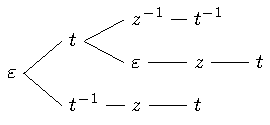
\includegraphics{figures/geodesicGenerating/treeRep}

	\caption{Tree representation of a geodesic equivalence class}
	\label{fig:tree1}
\end{figure}


Then, reading the nodes of the above tree from root to leaves, this tree represents the collection of words $tz^{-1}t^{-1}$, $tzt$, and $t^{-1}z t$.
Notice that each $\varepsilon$ is ignored when constructing words.

Given a tree of this form, the words can be extended a single letter in constant time.
For example, the words of the tree given earlier (in \cref{fig:tree1}) could be extended by the letter $z$ by adding a single edge to obtain the  tree in \cref{fig:tree2}, now rooted at $z$.

\begin{figure}[!ht]
	\centering

	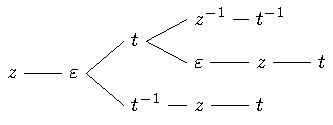
\includegraphics{figures/geodesicGenerating/treeRep2}

	\caption{The tree from \cref{fig:tree1}, extended by the letter $z$}
	\label{fig:tree2}
\end{figure}

Further, trees of this form can be combined (i.e.\ their words combined into one collection) in constant time, by adding two edges and a single node.
For example, consider the following union shown in \cref{fig:tree3}.

\begin{figure}[h!]
\begin{center}
	\begin{tabular}{m{3.5cm} m{1em} m{3.5cm} m{2em} m{4.5cm}}
		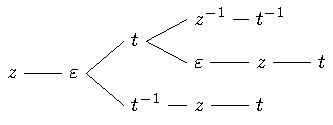
\includegraphics[width=3.5cm]{figures/geodesicGenerating/treeRep2}
		&
		\hfill
		$\bigcup$
		\hfill
		&
		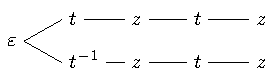
\includegraphics[width=3.5cm]{figures/geodesicGenerating/treeRep3}
		&
		\hfill
		$\Longrightarrow$
		\hfill
		&
		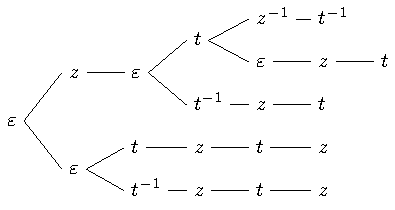
\includegraphics[width=4.5cm]{figures/geodesicGenerating/treeRep4Combined}
	\end{tabular}
\end{center}
\caption{Union of two rooted trees.}
	\label{fig:tree3}
\end{figure}


Thus, collections of words can be represented as tuples of the form $(w,B,T)$ where $w \in X^\ast$ is a representative of the collection, $B \subseteq X$ is the list of letters which begin words in the collection, and $T$ is a rooted tree as described earlier.
Using such tuples, it can be seen that collections of length $n-1$ geodesic can be extended to a collection of length $n$ words in constant time.
Thus, the list of length $n$ words can be produced in time $O(s(n-1))$, rather than $O(S(n-1))$.
Hence, it will be taken that $f(n) = 2 \cdot s(n-1)$ where $f(n)$ is as described at the beginning of this section, and $2 \cdot s(n-1)$ is an upper bound on the number of collections of extended words.

\begin{remark}
	It would also be possible to use tuples of the for $(w,B,\ell)$ where $\ell\in \mathbb{N}_+$ is the size (i.e.\ number of words) of the collection.
	This form does not contain enough information to recover the list full list of geodesics in each collection, however, it would contain enough compute the geodesic growth as the sum of all such $\ell$'s in the output.
	\thmendmark
\end{remark}

Notice that in the worst case, with respect to time complexity, all geodesics of length $n-1$ can be extended to length $n$ words as in \cref{rmk:genrated-next-geodesics}.
Thus, the variable $k$, which was used to denote the number of length $n$ input words, is bounded from above by $2 \cdot s(n-1)$.

Thus, the time-complexity of the full brute force algorithm is
\[
  O\left(
    \sum_{\ell = 1}^n \Big( 2 \cdot s(\ell-1) + (2 \cdot s(\ell-1))^2 \ell \log \ell \Big)
  \right)
  =
  O\left(
    \gamma(n-1)
    +
    \sum_{\ell=1}^n s(\ell-1)^2 \, \ell \log \ell
  \right)
\]
Then, considering that $s(\ell-1) \leq s(\ell-1)^2 \ell \log \ell$ and that $\sum_{\ell=1}^n s(\ell-1) = \gamma(\ell-1)\geq \gamma(\ell-1)$ it can be seen that this time complexity can be simplified to
\[
  O\left(
    \sum_{\ell=1}^n s(\ell-1)^2 \, \ell \log \ell
  \right)
\]
The time-complexity of the full sort-based algorithm is
\[
  O\left(
    \sum_{\ell = 1}^n \Big(
        2 \cdot s(\ell-1)
        +
        \big[2 \cdot s(\ell-1)\log (2 \cdot s(\ell-1)) + 2 \cdot s(\ell-1)\big] \, \ell \log \ell 
    \Big)
  \right)
\]
which can then be simplified to
\[
	O\left(
	\gamma(n-1)
	+
	\sum_{\ell = 1}^n
	\big[2 \cdot s(\ell-1)\log (2 \cdot s(\ell-1)) + 2 \cdot s(\ell-1)\big] \, \ell \log \ell
	\right)
\]
Then, simplified to
\[
O\left(
\gamma(n-1)
+
\sum_{\ell = 1}^n s(\ell-1) \log s(\ell-1) \, \ell \log \ell
\right)
\]
Then, considering that $\sum_{\ell = 1}^n s(\ell-1) \log s(\ell-1) \, \ell \log \ell$ grows faster, asymptotically, then $\gamma(n-1)$, it can be seen that this complexity becomes
\[
O\left(
\sum_{\ell = 1}^n s(\ell-1) \log s(\ell-1)  \, \ell \log \ell
\right)
\]
Hence, the complexity of the brute force and sorting based methods are
\begin{align*}
  O\left(
  \sum_{\ell=1}^n s(\ell-1)^2 \, \ell \log \ell
  \right)
  &&\text{and}&&
  O\left(
  \sum_{\ell = 1}^n s(\ell-1) \log s(\ell-1) \, \ell \log \ell
  \right)
\end{align*}
respectively.

Thus, it can be seen that the sorting-based method provides a better time complexity then the brute force method, particularly when considering that $s(n)$ is superpolynomial in complexity \cite{OnGrowth}.
To see this improvement, consider the following example.

\begin{example}
	For the moment suppose that $s(n) = e^{\sqrt{n}}$.
	Then, the respective complexities of the brute force and sort-based methods would be
	\begin{align*}
	O\left(
	\sum_{\ell=1}^n e^{2 \sqrt{\ell-1}} \, \ell \log \ell
	\right)
	&&\text{and}&&
	O\left(
	\sum_{\ell = 1}^n e^{\sqrt{\ell-1}} \sqrt{\ell-1} \, \ell \log \ell
	\right)
	\end{align*}
	Now, consider the following
	\[
	  \frac
	  {\displaystyle \sum_{\ell=1}^n e^{2 \sqrt{\ell-1}} \, \ell \log \ell}
	  {\displaystyle  \sum_{\ell = 1}^n e^{\sqrt{\ell-1}} \sqrt{\ell-1} \, \ell \log \ell}
	  \geq
	  \frac
	  {\displaystyle e^{2 \sqrt{n-1}} \, n \log n}
	  {\displaystyle n \cdot \left( e^{\sqrt{n-1}} \sqrt{n-1} \, n \log n \right) }
	  \geq
	  e^{\sqrt{n-1}} / n^2
	\]
	Thus, the worst-case sorting based method is (asymptotically) faster than the worst-case brute force method by, at least, a factor that is a multiple of $e^{\sqrt{n-1}}/n^2$, which is itself superpolynomial.
	
	Further, it is known from \cite{OnGrowth} that the complexity of $s(n)$ is higher than that of $e^{\sqrt{n}}$, and thus the difference in (worst-case) time complexity would be even more pronounced for Fabrykowski-Gupta.
\end{example}

\begin{remark}
	Both the brute force and sorting based methods have been implemented, by the author, in the programming language C.
	In less than two minutes, the sort-based method generated more data than the brute force method could in two weeks.
	Further, in less than ten hours the sort-based method was able to generate more data than the brute force method would be able to if it were given five centuries of time to run.
\end{remark}

